
\documentclass{acm_proc_article-sp}
\usepackage{float}
\begin{document}

\title{Multi-Market Deal Size Prediction}


\numberofauthors{1} %  in this sample file, there are a *total*
% of EIGHT authors. SIX appear on the 'first-page' (for formatting
% reasons) and the remaining two appear in the \additionalauthors section.
%
\author{
% 1st. author
\alignauthor
Evelin C. F. de Amorim \\
       \affaddr{Departamento de Ci\^{e}ncia da Computa\c{c}\~{a}o}\\
       \affaddr{Universidade Federal de Minas Gerais}\\
       \email{evelinamorim@ufmg.br}
}

\maketitle
\begin{abstract}

Daily-deals sites (DDSs) are web portals that offer discount coupons for services 
or products. Thus, customers are attracted by the captivate discounts. 
DDSs gain profit by the amount of coupons sold and  merchants, who offer  
services and products, gain profit by increasing the amount of clients 
. However, DDSs know 
beforehand the number of coupons sold, can benefit featured offers and 
bussiness strategies.

\emph{Deal size prediction} is the name of the task that predicts the number 
of coupons sold in a given offer. Some research proposed descriptive models 
to deal size, nonetheless few attempts have been made in order to 
predict deal size. Due to its practical importance, we propose a 
novel method to predict deal size. This method is based on an existing method, 
which considers latent markets in given catalog of deals. The existing method 
assigns only one latent market for a deal, and we propose to 
assign the deal to the most likely markets.

We perform experiments in order to detect 
only error in regression phase. The competition model is still in 
development, but we explain the competition model we intend to 
implement
. The results show evidences that 
include all probable markets,  
for a given deal, increase error. Also, we test another strategy that 
consider only markets with at least 0.3 of probability to own a given deal.

%the results balbla
\end{abstract}

% A category with the (minimum) three required fields
%\category{H.4}{Information Systems Applications}{Miscellaneous}
%A category including the fourth, optional field follows...
%\category{D.2.8}{Software Engineering}{Metrics}[complexity measures, performance measures]

%\terms{Theory}

%\keywords{ACM proceedings, \LaTeX, text tagging} % NOT required for Proceedings

\section{Introduction}

Daily-deals sites (DDSs) are popular web portals that offer discount coupons 
for services or products. These coupons includes expiration date, therefore 
it is not available for new customers acquire after a short period of time. 
As DDSs coupons are available for limited time, it is usual customers 
miss coupons. Also, customers have decided soon which coupon to buy. 
Considering that the customers own a limited budget, some coupons 
will be disregarded in favor of others coupons.

Coupons that provide similar services or products can bring doubt to 
consumer mind. Thefore, the number of coupons sold of one deal  
can affect the number of coupons sold of another similar deal. From this ideia, 
Lacerda et. al ~\cite{lacerda2014context} proposed a 
strategy, called \emph{Competitive Business Market Prediction} 
(CPMB),
that assigns each deal in the DDS catalog to a latent 
market. CPMB strategy is composed by three main steps:
the first step divides the catalog of deals into markets 
by using Latent Dirichlet Allocation (LDA); the second step perfoms 
regression training in each market; and the third step executes an 
expectation-maximization  procedure in order to consider the 
competition among the deals in the same market.

Byers et. al ~\cite{BMZ12} performed an experiment in order to evaluate 
the impact of online social network in the sales of discount coupons 
of DDSs. Also, Byers builds a linear model to depict the deal size 
according to the deal features. The authors conclude that predicting 
deal size is challenging and future research can explore merchant information 
from reviews web sites.

Although there is practical importance of deal size prediction task, 
there are a minimal amount of research. For these reason, we proposed 
a method based on Lacerda's research in order to achieve better results. 
Nevertheless, our proposal supposes that deals can belong to more than 
one market. %the results balbla

\section{Methodology}

The methodology that we propose is comprised by three steps: 
separation of the deals of the catalog into markets, regression training 
of the deals, and expectation-maximization of the deals in the same 
market. Althought, our steps are very similar to Lacerda's steps, 
the first step is modified in order to assign each offer to the 
most likely markets.

The following subsections explain the methodology in details and 
the evaluation metric employed to evaluate our results.

\subsection{Algorithm}

The algorithm is composed by three phases: Market identification, 
Regression per Market, and Market Weighting. Next, we will 
describe how these three phases are implemented.

\textbf{Market Identification.} Each deal presents textual features 
like: title, description, 
merchant, and so on. These textual features are extracted 
of each deal and tokenized. \texttt{NLTK}\footnote{www.nltk.org} library 
performs the tokenization of each textual feature of a deal. 
Next, stop words are removed and a stemmer are applied to tokens. 
Both stop words and stemmer processes are perfomed by 
\texttt{NLTK} library, which provides a constant list of words 
for stop words and the Porter's algorithm for stemming.
Also common tokens in the catalog is removed, by common tokens 
we consider tokens that appear in at least 25\%  of documents.

After process textual features,
Latent Dirichlet Allocation (LDA) 
method is applied in order to identified the markets. LDA method 
build probabilistic distributions in order to infer latent topics 
in a given collection. The probabilistic distribution are assemble 
based on a weight, which can be, for instance, term frequency in 
the document. The weigthing scheme in this research is 
\emph{term spread}, which is defined by the Equation 
\ref{eq:termspread}.

\begin{equation}
    TS(t,d) = \sum_{s \in d} i, \text{where i} \left\{ \begin{aligned} 
    1 & & t \in s \\
    0 & & otherwise \\
    \end{aligned} \right.
    \label{eq:termspread}
\end{equation}


The implementation of LDA executed in experiments is from 
{\v R}eh{\r u}{\v r}ek and Petr Sojka ~\cite{rehureklrec}.
%explicar que features textuais podem ter uma deal

\textbf{Regression per Market.} After the processing of textual features, 
each deal is assigned to 
the most probable markets. Next, one regression model is trained 
in historical data for each market. The regression method is trained in the 
following deal features:

\begin{itemize}
    \item City of the deal;
    \item The absolute value of the discount;
    \item Wether the deal sold out;
    \item Number of the days which the deal is available for costumers;
    \item Day of week that the deal starts;
    \item Category in the DDS web site.
\end{itemize}


Each regression model predicts 
the deals of the test set, whether one deal belongs to more than one 
market, then a weighted mean is computed according to Equation \ref{wpred}, 
where $\sigma(d,t)$ is the predicted value for the deal $d$, if the deal 
belongs to market $t$.

\begin{equation}
    pred(d) = \sum_{d \in S} p(S)\times \sigma(d,S)
    \label{wpred}
\end{equation}

Prediction step is applied 
only to deals of the day and we employ and SVR as 
regression method. 
There are as many classifiers as latent markets.

\textbf{Market Weighting}. After the building of regressor classifiers, 
weights are computed to consider the impact of the market in deal size 
prediction. The processes of compute market weights starts with the partition of 
the catalog into $k$ markets, so that $S =\{S_{m_1},S_{m_2},\cdots,S_{m_k}\}$.
Each deal $q \in S$ belongs to one or more markets, and we call $S_q$ the 
subset of markets that owns $q$. Again, in these step we consider the 
prediction as an weigthted mean of predictions. For each market $S^{j}_q \in S_q$ 
we compute the Equation \ref{sigma}.

\begin{equation}
    \sigma^j(q) = \alpha \times \frac{\sum\limits_{\forall d^j \in S^j_q} f(d^j) \times \rho(S^j_q)}{|S^j_q|} + (1 - \alpha) \times f(q)
    \label{sigma}
\end{equation}

The variable $\rho(S^j)$ is unknown and is estimated by the  
expectation-maximization (EM) algorithm. The Equation \ref{rho} calculates $\rho$ 
in each iteration of EM procedure.

\begin{equation}
    \rho(S^j_q) = \frac{\sum_{\forall d^j \in S^j_q} \sigma(d^j)}{\sum_{\forall d \in S} \sigma(d)}
    \label{rho}
\end{equation}

Then, the prediction for a given deal $q$ is depicted by the weighted mean 
of $\sigma^j$ predictions for $q$. The weight is, again, the probability of $q$ 
belongs to the market $S^j_q$.

The loss function for the expectation-maximization is 
\emph{Root Mean Square Error}(RMSE), which is defined by Equation 
\ref{rmse}.

\begin{equation}
    RMSE(y,\sigma) = \sqrt{\frac{1}{n}\sum_{1\geq i}(y_i - sigma(q))^2}
    \label{rmse}
\end{equation}

, where $\sigma(q)$ is the weithed mean of $\sigma^j(q)$ and $n$ is the number 
of predicted deals.

\subsection{Evaluation}

There are many ways to evaluate recommender systems. However, our task 
is not the recommendation itself and but a support task for 
recommender systems. Also, the sizes of the deals can vary greatly and 
we model our problem as a regression problem.
For these reasons, we adopt the 
\emph{Root Relative Square Error} (RRSE)  as evaluation metric, which is 
defined by Equation \ref{rrse}. 

\begin{equation}
    RRSE(y,\hat{y}) = \sqrt{\frac{\sum_{i=1}^n (\hat{y_i}-y_i)^2}{\sum_{i=1}^n (\bar{y}-y_i)^2}}
    \label{rrse}
\end{equation}

, where $\hat{y_i}$ is the i-th predicted value, $\bar{y}$ is the mean of 
labels $y$ , and $n$ is the number of predicted values.

\section{Experiments and Results}

The implementation of this research produced a different outcome reported  
by the original~\cite{lacerda2014context}. The reasons for this outcome 
may vary: different parameters for griding search in SVR, different dataset, 
differences in the features of dataset, 
details about expectation-maximization from Lacerda's thesis, and so on.
In face os these issues, we performed alternative experiments. The following 
sections describe the dataset employed and the experiments performed.


\subsection{Dataset}

Dataset employed in the experiments was provided by Byers et. al ~\cite{BMZ12}.
There are two DDSs web portal in Byer's collection: Groupon and Living Social. 
As we demand textual features, and Byers collection's has only structural 
features of the deals, we crawled the web pages from mentioned DDSs portals. 
Nonetheless, some deals are unavailable, therefore the number of the deals 
we tested is different from the numbers reported by Byers.


The deals from living social dataset were collected between March 21st and 
July 3rd, 2011. The textual features from these dataset were crawled in 
September 24th, 2014. From the original dataset, we excluded 19 deals, 
resulting in 2590 deals. The deals from groupon were not tested, due to 
time constranints. We depicted the distribution of deal size of 
both datasets in Figure \ref{dealsize}. The distributions of deal 
sizes resemble an exponential distribution: few deals with low deals sizes 
and the most of them between median and the maximum value.

\begin{figure}[H]
    \centering
    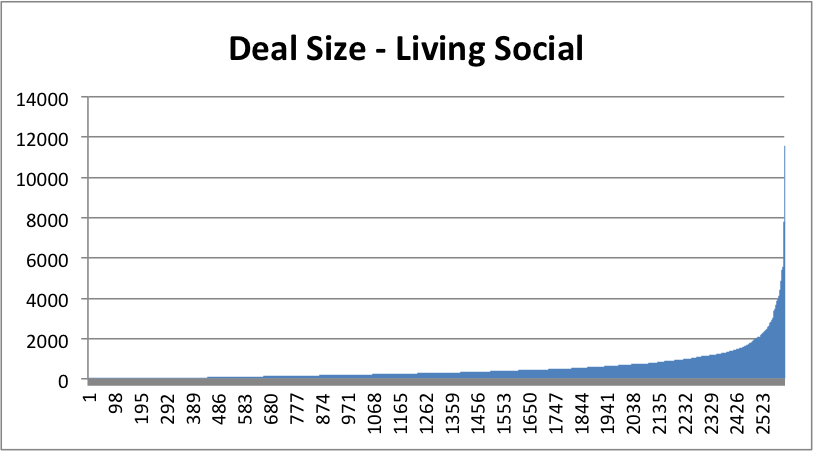
\includegraphics[scale=0.5]{dealsizels.png}
    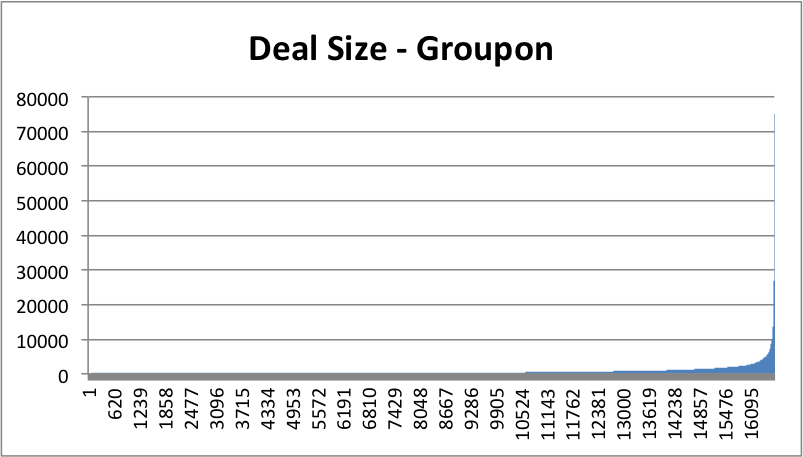
\includegraphics[scale=0.5]{dealsizegroupon.png}
    \caption{Distribution of Deal Size in the Dataset}
    \label{dealsize}
\end{figure}


\subsection{Experiments}

Due to the time constraints and difficulties in the interpretation of 
the description of the strategy, it was not possible perform the 
experiments as we wish. 

%guidelines
%1
Larcerda employed an SVR classifier for each market and then 
an EM method. Also, in the Larceda's research was performed 
a grid search for find the best SVR classifier for each market and 
and SVR rbf kernel was employed. However, we considered linear 
kernel for grid search as well. The linear kernel performs  
efficientle in datasets that are linearly. The parameters for 
our grid search was $C = \{0.01,0.1,$$1,5,10,50\}$ and 
$\gamma = \{0,0.001,0.0000001\}$.


%2
The EM procedure was not clear in the Lacerda's P.h.d. thesis. The definition of 
the EM method ~\cite{hastie2009elements} comprises the likelihood 
of an mixture statiscal distribution. However, the definition 
provided is unclear whether the likelihood is applied in the 
method. Although the description of the discovery of the 
marketing competition is vague, we attemped to implement 
the procedure described. Nevertheless, we failed in reproducing 
the EM step.

Despite of the problems in reproducing Larceda's research, we 
attempt to evaluate the  RRSE for SVR strategy. The ideia is 
to test the hypothesis that employing best market to 
predict deal size can be improved considering all the possible 
market or considering the markets above a threshold.

Table \ref{rmsetable} shows the best results for the best market, 
all markets and threshold market. The threshold tested was $0.3$, i.e., 
only the markets that has the probility of $0.3$ or above to 
own one given deal is considered in the weighted mean of such deal.

\begin{table}[H]
    \centering
    \caption{RRSE for all the strategies and 30 markets}
    \label{rmsetable}
    \begin{tabular}{lc} \hline
	Strategy & RRSE \\ \hline \hline
	Best & 1.03\\
        All & 1.13 \\
	Threshold & 1.06 \\ \hline
    \end{tabular}
\end{table}

The results we obtain are slightly better that Lacerda reports, 
however our dataset is different and we also experimented 
linear kernel in our grid search. 

The Figure ~\cite{rrsemarkets} shows a graph for the evolution 
of the error 
for \emph{All} strategy and \emph{Threshold} strategy. The behavior of 
both strategies are similar to the Lacerda's strategy. We observe that 
the behavior of \emph{Best} strategy is consistently better 
than \emph{All} strategy. While the \emph{threshold} strategy is better 
than \emph{All} strategy. The \emph{Best} strategy perform better than 
the other two strategies.

\begin{figure}[H]
    \centering
    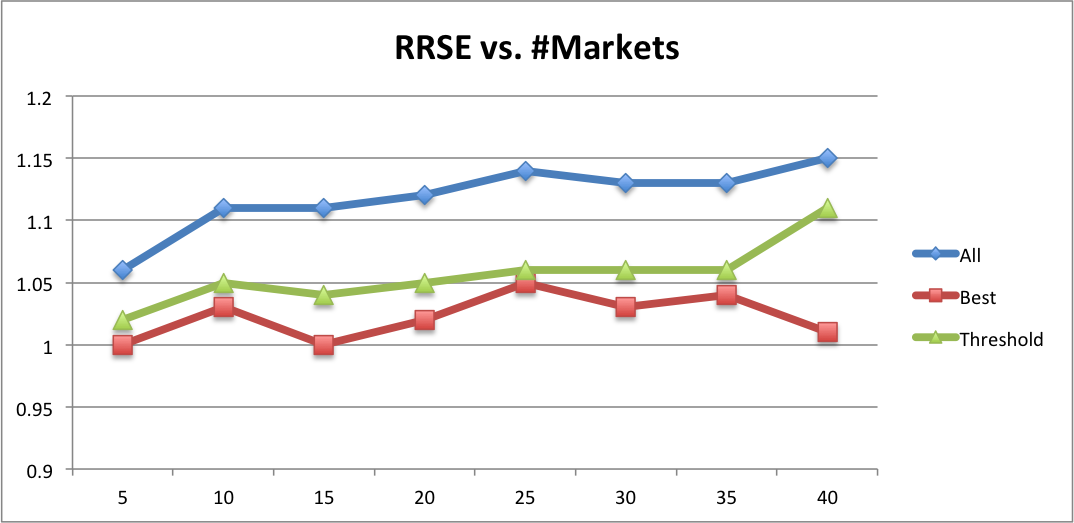
\includegraphics[scale=0.5]{rrsemarkets.png}
    \caption{RRSE vs. \#Markets}
    \label{rrsemarkets}
\end{figure}

Our experiments were performed without compute confidence interval and 
another statistical tests. As we consider these experiments only 
as initial results, we intend to perform carefully tests in order 
to corroborate the results from initial experiments.

\section{Conclusion and Discussion}

We proposed a modification in Lacerda's research in order to 
obtain better results. However, our strategy seens simple 
to consider the participation of one deal in different markets. 
It is possible that the errors of all markets 
 introduce more errors in the final result. 
 
 More tests must be perfomed  as well. The groupon dataset was not 
 tested and more tests can produce more insightful clues about 
 more sophisticate techniques, that can consider multi-market deals 
 but avoid to introduce errors like the strategy proposed here. 

 Although the strategy here may be introducing errors in the 
 regression prediction, we may investigate whether is this really 
 the case.

Also, the vague description of the expectation-maximization strategy 
of Lacerda's P.h.d. thesis, become difficult to implement 
the strategy in time. Maybe if we employ the multi-market 
strategy in EM algorithm, the outcome can be improved, even though 
 the multi-market strategy 
performed worse compared to best-market for the regression 
module.

More experiments are being made, like the variation in the 
threshold of the \emph{threshold} strategy. Therefore this report will be 
incremented with new information.
%
% The following two commands are all you need in the
% initial runs of your .tex file to
% produce the bibliography for the citations in your paper.
\bibliographystyle{abbrv}
\bibliography{sigproc}  % sigproc.bib is the name of the Bibliography in this case
% You must have a proper ".bib" file
%  and remember to run:
% latex bibtex latex latex
% to resolve all references
%
% ACM needs 'a single self-contained file'!
%
%APPENDICES are optional
%\balancecolumns
\end{document}
